\chapter{\label{cpt:architecture}Architecture}

The architecture of \Amber\ is defined in terms of modules, whiteboards and the
messages they use to communicate. Figure~\ref{fig:global-architecture} shows
the flow of messages between the modules and whiteboards.

In the Section~\ref{sct:modules} the modules are described and in
Section~\ref{sct:messages} the messages connecting them are defined. % The data
% types used in the system are described in Section~\ref{sct:types}.

\begin{figure}
    \centering
    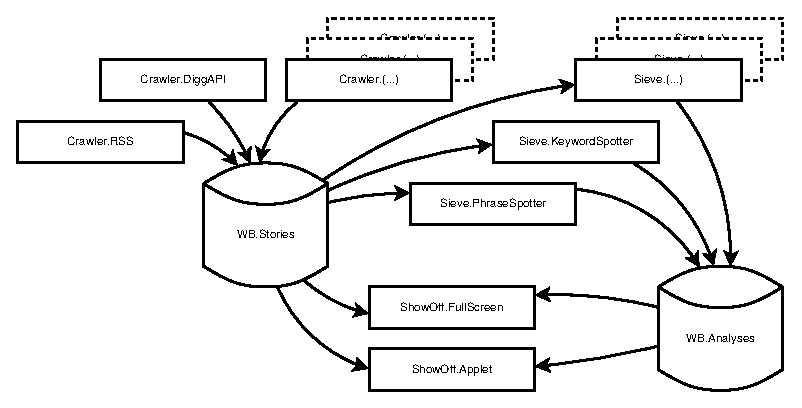
\includegraphics{\designpath/image/global-architecture}
    \caption{\label{fig:global-architecture}Global \Amber\ architecture, the
              names are Psyclone module names}
\end{figure}

\section{\label{sct:modules}Modules}

A complete \Amber\ system will comprise at least three modules running at the
same time; there is a Crawler module, an analysis module called Sieve and a
display called ShowOff. The modules are separate executables with their own
life-cycles and resources. Since TCP/IP is used, the executables don't need to
be on the same machine to communicate.

Every module has a specified interface through which communication with
Psyclone is handled.

\subsection{Crawler modules}

When the Crawler is started, it will create one of the available handlers
(depending on what is specified on the command line or what is set as default
during build time). 

It also creates an AirBrush instance to communicate with Psyclone via
Java\-Open\-AIR. The module name announced to Psyclone is `Crawler.' plus the
name of the handler, so `Crawler.RSS' in case of the RSS handler.

After connecting with Psyclone, the handler can get its parameters stored in
the psySpec file and go to work. It will post stories with type `Story'  on the
whiteboard `WB.Stories'.

\subsubsection{RSS}

The RSS crawler module will be fairly straightforward. It fetches the RSS feed
from a set URL and produces a Story message for every new item that appears.
The contents of the Story message is specified in Section~\ref{sct:messages}.

Although the module is called RSS, it can handle Atom feeds, which is also
quite a popular format.

\begin{module}{Crawler.RSS}
  \trigger{Feed.*}{WB.Control}
  \post{Story}{WB.Stories}
\end{module}

\subsubsection{DiggAPI}

Digg is a website which lets users submit stories found on the web. Other users
then moderate the submissions either by `digging' or `burying' a story. A story
with a lot of `diggs' is a popular one. The nice thing about Digg is that it
actually does a lot of preprocessing work for the \Amber\ system.

Digg
announced\footnote{\url{http://diggtheblog.blogspot.com/2006/07/digg-labs-launches-alpha.html}}
that they will publish a public API within the next months. If time allows, a
DiggAPI module is created.

\begin{module}{Crawler.DiggAPI}
    \post{Story}{WB.Stories}
\end{module}

% \subsubsection{BloggerDataAPI}
% 
% One of the larger weblog hosters is Google with their Blogger service. There
% is an API available to get information from it.
% 
% \begin{module}{Crawler.BloggerDataAPI}
%   \post{Story}{WB.Stories}
% \end{module}


\subsection{Sieve modules}

All analysis modules, or sieves, will get a trigger from a new story on the
whiteboard WB.Stories. They analyse it and if it can say anything about the
story, an Analysis message is sent to the whiteboard WB.Analyses containing its
judgement on the story.

The contents of this message is specified in Section~\ref{sct:messages}.

Analysis modules may take any time they like to come to a verdict, but it is
possible that a story has already disappeared from the visualization if the
response is very late.

Since all modules regardless of their functionality employ the same external
behaviour, the Psyclone specification is the same for every one of them.

\begin{module}{Sieve.???}
    \trigger{Story}{WB.Stories}
    \post{Analysis}{WB.Analyses}
\end{module}

\subsection{ShowOff modules}

The ShowOff modules are visualizers which combine the crawled stories from the
Crawler with the analyses from the Sieve modules.

\begin{module}{ShowOff.???}
    \trigger{Story}{WB.Stories}
    \trigger{Analysis}{WB.Analyses}
\end{module}

\subsubsection{Full screen}

The full screen application will display a lot of information and is there to
be looked - not glanced - at. It should be possible to let it do its job
autonomously, just showing a pretty picture, or to be interactive.

\subsubsection{Ambient applet}

The ambient applet will display a very easy to understand image (a glance at it
should be enough) of the status of the page it is on. I.e. if the page is a
weblog, it should display subject information on that weblog, if it is on the
page of a thread of a forum, it displays the flow of the discussion.



\section{\label{sct:messages}Messages}

FIXME: Add life-cycle model of amber.Story.


\subsection{Between Crawler and Sieve}


\subsection{Between Sieve and ShowOff}




% \section{\label{sct:types}Data types}

\subsection{Story}

The story type holds the text of an entry, plus meta-data. It is a shared type
between all three modules and it is also exported to the Psyclone whiteboards.

% \begin{type}
  % 
% \end{type}


